% Options for packages loaded elsewhere
\PassOptionsToPackage{unicode}{hyperref}
\PassOptionsToPackage{hyphens}{url}
%
\documentclass[
]{article}
\usepackage{amsmath,amssymb}
\usepackage{iftex}
\ifPDFTeX
  \usepackage[T1]{fontenc}
  \usepackage[utf8]{inputenc}
  \usepackage{textcomp} % provide euro and other symbols
\else % if luatex or xetex
  \usepackage{unicode-math} % this also loads fontspec
  \defaultfontfeatures{Scale=MatchLowercase}
  \defaultfontfeatures[\rmfamily]{Ligatures=TeX,Scale=1}
\fi
\usepackage{lmodern}
\ifPDFTeX\else
  % xetex/luatex font selection
\fi
% Use upquote if available, for straight quotes in verbatim environments
\IfFileExists{upquote.sty}{\usepackage{upquote}}{}
\IfFileExists{microtype.sty}{% use microtype if available
  \usepackage[]{microtype}
  \UseMicrotypeSet[protrusion]{basicmath} % disable protrusion for tt fonts
}{}
\makeatletter
\@ifundefined{KOMAClassName}{% if non-KOMA class
  \IfFileExists{parskip.sty}{%
    \usepackage{parskip}
  }{% else
    \setlength{\parindent}{0pt}
    \setlength{\parskip}{6pt plus 2pt minus 1pt}}
}{% if KOMA class
  \KOMAoptions{parskip=half}}
\makeatother
\usepackage{xcolor}
\usepackage[margin=1in]{geometry}
\usepackage{color}
\usepackage{fancyvrb}
\newcommand{\VerbBar}{|}
\newcommand{\VERB}{\Verb[commandchars=\\\{\}]}
\DefineVerbatimEnvironment{Highlighting}{Verbatim}{commandchars=\\\{\}}
% Add ',fontsize=\small' for more characters per line
\usepackage{framed}
\definecolor{shadecolor}{RGB}{248,248,248}
\newenvironment{Shaded}{\begin{snugshade}}{\end{snugshade}}
\newcommand{\AlertTok}[1]{\textcolor[rgb]{0.94,0.16,0.16}{#1}}
\newcommand{\AnnotationTok}[1]{\textcolor[rgb]{0.56,0.35,0.01}{\textbf{\textit{#1}}}}
\newcommand{\AttributeTok}[1]{\textcolor[rgb]{0.13,0.29,0.53}{#1}}
\newcommand{\BaseNTok}[1]{\textcolor[rgb]{0.00,0.00,0.81}{#1}}
\newcommand{\BuiltInTok}[1]{#1}
\newcommand{\CharTok}[1]{\textcolor[rgb]{0.31,0.60,0.02}{#1}}
\newcommand{\CommentTok}[1]{\textcolor[rgb]{0.56,0.35,0.01}{\textit{#1}}}
\newcommand{\CommentVarTok}[1]{\textcolor[rgb]{0.56,0.35,0.01}{\textbf{\textit{#1}}}}
\newcommand{\ConstantTok}[1]{\textcolor[rgb]{0.56,0.35,0.01}{#1}}
\newcommand{\ControlFlowTok}[1]{\textcolor[rgb]{0.13,0.29,0.53}{\textbf{#1}}}
\newcommand{\DataTypeTok}[1]{\textcolor[rgb]{0.13,0.29,0.53}{#1}}
\newcommand{\DecValTok}[1]{\textcolor[rgb]{0.00,0.00,0.81}{#1}}
\newcommand{\DocumentationTok}[1]{\textcolor[rgb]{0.56,0.35,0.01}{\textbf{\textit{#1}}}}
\newcommand{\ErrorTok}[1]{\textcolor[rgb]{0.64,0.00,0.00}{\textbf{#1}}}
\newcommand{\ExtensionTok}[1]{#1}
\newcommand{\FloatTok}[1]{\textcolor[rgb]{0.00,0.00,0.81}{#1}}
\newcommand{\FunctionTok}[1]{\textcolor[rgb]{0.13,0.29,0.53}{\textbf{#1}}}
\newcommand{\ImportTok}[1]{#1}
\newcommand{\InformationTok}[1]{\textcolor[rgb]{0.56,0.35,0.01}{\textbf{\textit{#1}}}}
\newcommand{\KeywordTok}[1]{\textcolor[rgb]{0.13,0.29,0.53}{\textbf{#1}}}
\newcommand{\NormalTok}[1]{#1}
\newcommand{\OperatorTok}[1]{\textcolor[rgb]{0.81,0.36,0.00}{\textbf{#1}}}
\newcommand{\OtherTok}[1]{\textcolor[rgb]{0.56,0.35,0.01}{#1}}
\newcommand{\PreprocessorTok}[1]{\textcolor[rgb]{0.56,0.35,0.01}{\textit{#1}}}
\newcommand{\RegionMarkerTok}[1]{#1}
\newcommand{\SpecialCharTok}[1]{\textcolor[rgb]{0.81,0.36,0.00}{\textbf{#1}}}
\newcommand{\SpecialStringTok}[1]{\textcolor[rgb]{0.31,0.60,0.02}{#1}}
\newcommand{\StringTok}[1]{\textcolor[rgb]{0.31,0.60,0.02}{#1}}
\newcommand{\VariableTok}[1]{\textcolor[rgb]{0.00,0.00,0.00}{#1}}
\newcommand{\VerbatimStringTok}[1]{\textcolor[rgb]{0.31,0.60,0.02}{#1}}
\newcommand{\WarningTok}[1]{\textcolor[rgb]{0.56,0.35,0.01}{\textbf{\textit{#1}}}}
\usepackage{longtable,booktabs,array}
\usepackage{calc} % for calculating minipage widths
% Correct order of tables after \paragraph or \subparagraph
\usepackage{etoolbox}
\makeatletter
\patchcmd\longtable{\par}{\if@noskipsec\mbox{}\fi\par}{}{}
\makeatother
% Allow footnotes in longtable head/foot
\IfFileExists{footnotehyper.sty}{\usepackage{footnotehyper}}{\usepackage{footnote}}
\makesavenoteenv{longtable}
\usepackage{graphicx}
\makeatletter
\def\maxwidth{\ifdim\Gin@nat@width>\linewidth\linewidth\else\Gin@nat@width\fi}
\def\maxheight{\ifdim\Gin@nat@height>\textheight\textheight\else\Gin@nat@height\fi}
\makeatother
% Scale images if necessary, so that they will not overflow the page
% margins by default, and it is still possible to overwrite the defaults
% using explicit options in \includegraphics[width, height, ...]{}
\setkeys{Gin}{width=\maxwidth,height=\maxheight,keepaspectratio}
% Set default figure placement to htbp
\makeatletter
\def\fps@figure{htbp}
\makeatother
\setlength{\emergencystretch}{3em} % prevent overfull lines
\providecommand{\tightlist}{%
  \setlength{\itemsep}{0pt}\setlength{\parskip}{0pt}}
\setcounter{secnumdepth}{-\maxdimen} % remove section numbering
\usepackage{float}
\usepackage{booktabs}
\usepackage{longtable}
\usepackage{array}
\usepackage{multirow}
\usepackage{wrapfig}
\usepackage{colortbl}
\usepackage{pdflscape}
\usepackage{tabu}
\usepackage{threeparttable}
\usepackage{threeparttablex}
\usepackage[normalem]{ulem}
\usepackage{makecell}
\usepackage{xcolor}
\ifLuaTeX
  \usepackage{selnolig}  % disable illegal ligatures
\fi
\IfFileExists{bookmark.sty}{\usepackage{bookmark}}{\usepackage{hyperref}}
\IfFileExists{xurl.sty}{\usepackage{xurl}}{} % add URL line breaks if available
\urlstyle{same}
\hypersetup{
  hidelinks,
  pdfcreator={LaTeX via pandoc}}

\author{}
\date{\vspace{-2.5em}}

\begin{document}

\hypertarget{how-did-rotation-system-and-corn-weed-management-affect-crop-yields}{%
\paragraph*{How did rotation system and corn weed management affect crop yields?}\label{how-did-rotation-system-and-corn-weed-management-affect-crop-yields}}
\addcontentsline{toc}{paragraph}{How did rotation system and corn weed management affect crop yields?}

Results of the experiment indicated that crop diversification and reduced use of herbicides were not associated with lower crop yields (Table \ref{tab:crop-jt-ct}). Averaged over four years, soybean was the only crop whose yield was affected by rotation (p = 0.0191, Table \ref{tab:crop-jt-ct}). Soybean yield was 16\% higher in the 4-year rotation than in the 2-year rotation (p = 0.0181). Crop yields in the experiment were as high or higher than the averages for the state of Iowa and Boone County (Figure \ref{fig:crop-bar}).

\begin{table}

\caption{\label{tab:crop-jt-ct}Contrasts of rotation effect (expressed by Crop ID) on crop yields. The abbreviations on the contrast column are crop identities, which are the combinations of the first letter in crop species names and the rotation in which it occurred.}
\centering
\begin{threeparttable}
\begin{tabular}[t]{lrrr>{}r|lrr}
\toprule
\multicolumn{5}{c}{ANOVA} & \multicolumn{3}{c}{Comparison} \\
\cmidrule(l{3pt}r{3pt}){1-5} \cmidrule(l{3pt}r{3pt}){6-8}
Source of variation & df1 & df2 & F & p & contrast & ratio & p\\
\midrule
\addlinespace[0.3em]
\multicolumn{8}{l}{\textbf{(A) - Corn}}\\
\hspace{1em}Crop ID & 2 & 6 & 3.19 & 0.1138 & C2 vs C3 & 0.94 & 0.1882\\
\hspace{1em}Corn weed management & 1 & 3 & 0.32 & 0.6088 & C2 vs C4 & 0.93 & 0.1278\\
\hspace{1em}Crop ID x Corn weed management & 2 & 6 & 2.20 & 0.1914 & C3 vs C4 & 0.99 & 0.9507\\
\addlinespace[0.3em]
\multicolumn{8}{l}{\textbf{(B) - Soybean}}\\
\hspace{1em}Crop ID & 2 & 6 & 8.22 & 0.0191 & S2 vs S3 & 0.96 & 0.5499\\
\hspace{1em}Corn weed management & 1 & 3 & 0.18 & 0.7018 & S2 vs S4 & 0.86 & 0.0181\\
\hspace{1em}Crop ID x Corn weed management & 2 & 6 & 0.62 & 0.5678 & S3 vs S4 & 0.90 & 0.0670\\
\addlinespace[0.3em]
\multicolumn{8}{l}{\textbf{(C) - Oat}}\\
\hspace{1em}Crop ID & 1 & 2 & 1.35 & 0.3647 & O3 vs O4 & 0.91 & 0.3647\\
\bottomrule
\end{tabular}
\begin{tablenotes}[para]
\item \textit{Note: } 
\item Corn weed management: low herbicide or conventional. Crop ID: crop species and the cropping system in which it occurred: C2 - corn in the 2-year rotation, C3 - corn in the 3-year rotation, C4 - corn in the 4-year rotation, S2 - soybean in the 2-year rotation, S3 - soybean in the 3-year rotation, S4 - soybean in the 4-year rotation, O3 - oat in the 3-year rotation, and O4 - oat in the 4-year rotation.
\end{tablenotes}
\end{threeparttable}
\end{table}

\begin{figure}
\centering
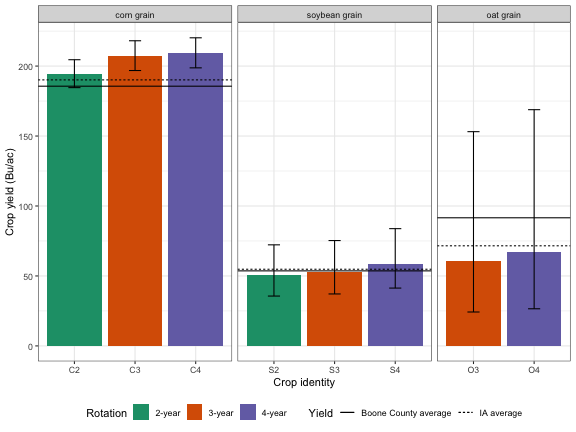
\includegraphics{Crop_yields_bushel_files/figure-latex/crop-bar-1.png}
\caption{\label{fig:crop-bar}Mean crop yields by rotation from 2017 to 2020. The color-coded bars show crop yields (Mg ha\(^-1\)) in the experiment plots. The error bars show the 95\% confidence intervals. The solid horizontal lines show mean yields for Iowa and dashed lines show mean yields for Boone County. Corn, soybean, and alfalfa yields in the experiment were averaged over four years, oat grain yields in the experiment were averaged over 2017, 2019, and 2020 because in 2018 oat was harvested for hay. Boone County and Iowa hay yields were averaged over 2017 and 2018 because 2019 and 2020 yields were not available at this writing.}
\end{figure}

Why is Marsden hay yield in ton/ac lower than IA and Boone averages, while yield in Mg/ha higher?

\begin{Shaded}
\begin{Highlighting}[]
\NormalTok{crops.emmip.IA }\SpecialCharTok{\%\textgreater{}\%}
  \FunctionTok{filter}\NormalTok{(Commodity }\SpecialCharTok{==} \StringTok{"alfalfa hay"}\NormalTok{) }\SpecialCharTok{\%\textgreater{}\%}
\FunctionTok{ggplot}\NormalTok{(}\FunctionTok{aes}\NormalTok{(}\AttributeTok{x =}\NormalTok{ Crop\_ID, }\AttributeTok{y =}\NormalTok{ yvar, }\AttributeTok{fill =}\NormalTok{ Rotation))}\SpecialCharTok{+} 
  \FunctionTok{geom\_bar}\NormalTok{(}\AttributeTok{stat =} \StringTok{"identity"}\NormalTok{) }\SpecialCharTok{+}
  \FunctionTok{scale\_fill\_brewer}\NormalTok{(}\AttributeTok{palette =} \StringTok{"Dark2"}\NormalTok{) }\SpecialCharTok{+}
  \FunctionTok{geom\_errorbar}\NormalTok{(}\FunctionTok{aes}\NormalTok{(}\AttributeTok{ymin=}\NormalTok{ LCL, }\AttributeTok{ymax=}\NormalTok{ UCL), }\AttributeTok{width=}\NormalTok{.}\DecValTok{2}\NormalTok{) }\SpecialCharTok{+} 
  \FunctionTok{facet\_grid}\NormalTok{(.}\SpecialCharTok{\textasciitilde{}}\NormalTok{ Commodity, }\AttributeTok{scales =} \StringTok{"free"}\NormalTok{, }\AttributeTok{space =} \StringTok{"free"}\NormalTok{) }\SpecialCharTok{+} \CommentTok{\# scales: remove empty bar, space: equal bar width}
  \FunctionTok{geom\_hline}\NormalTok{(}\FunctionTok{aes}\NormalTok{(}\AttributeTok{yintercept =}\NormalTok{ IA\_avg\_Bu, }\AttributeTok{linetype =} \StringTok{"IA average"}\NormalTok{)) }\SpecialCharTok{+} 
  \FunctionTok{geom\_hline}\NormalTok{(}\FunctionTok{aes}\NormalTok{(}\AttributeTok{yintercept =}\NormalTok{ Boone\_avg\_Bu, }\AttributeTok{linetype =} \StringTok{"Boone County average"}\NormalTok{)) }\SpecialCharTok{+} 
  \FunctionTok{ylab}\NormalTok{(}\StringTok{"Crop yield (ton/ac)"}\NormalTok{) }\SpecialCharTok{+}
  \FunctionTok{xlab}\NormalTok{(}\StringTok{"Crop identity"}\NormalTok{) }\SpecialCharTok{+}
  \FunctionTok{labs}\NormalTok{(}\AttributeTok{linetype =} \StringTok{"Yield"}\NormalTok{) }\SpecialCharTok{+}
  \FunctionTok{theme}\NormalTok{(}\AttributeTok{legend.position=}\StringTok{"bottom"}\NormalTok{) }
\end{Highlighting}
\end{Shaded}

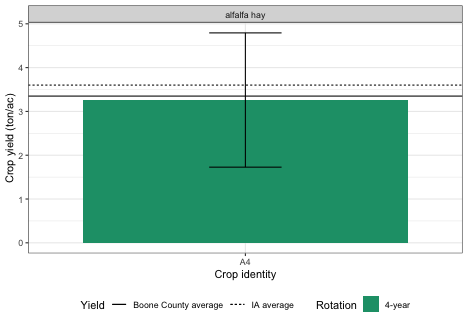
\includegraphics{Crop_yields_bushel_files/figure-latex/unnamed-chunk-8-1.png}

\end{document}
